\documentclass{article}
\usepackage[utf8]{inputenc}
\usepackage{amsthm}
\usepackage{amsmath}
\newtheoremstyle{mystyle}% name
  {\topsep}% Space above
  {\topsep}% Space below
  {\normalfont}% Body font
  {}% Indent amount
  {\bfseries}% Theorem head font
  {}%Punctuation after theorem head
  {.5em}%Space after theorem head
  {}% theorem head spec
\theoremstyle{mystyle}
\newtheorem{prob}{Problem}
\usepackage{graphicx}
\usepackage{wrapfig}
 %preamble
\title{Project 2}
\author{LJ Gonzales}
\date{April 2023}

\begin{document}
\maketitle
\section{Part I}
To encode the signals, we first find the correct frequencies according to the key input by use of what is effectively a dictionary: using the \emph{find} function on a list containing the keys outputs a value between 1 and 12, which is then used as an index for the "low frequency" and "high frequency" lists. 
We then instantiate \emph{x\_axis}, which represents the timepoints of the continuous sinusoidal that the discretized version will record as samples.
It is a linspace range beginning at 1, ending at the user parameter \emph{duration} (defaulted to 0.2 and measured in seconds), and with step $\frac{1}{fs}$, defaulted to 8000 in Hertz.
Two sinusoidals are generated, one by $sin(2\pi f\text{x\_axis})$, where f is the respective frequencies of low and high sinusoidal.
Finally, the function returns the weighted addition of these two sinusoidals, defaulting to 1,1 for the weights.
We verified the output quantitatively by comparing the tone with the ones produced by a Xiaomi Note 7 cellphone, which seems to use the standard DTMF. Possible variations in weighting aside, the tones sounded similar to the respective ones produced by DTMFencode.
\begin{figure}[h]
	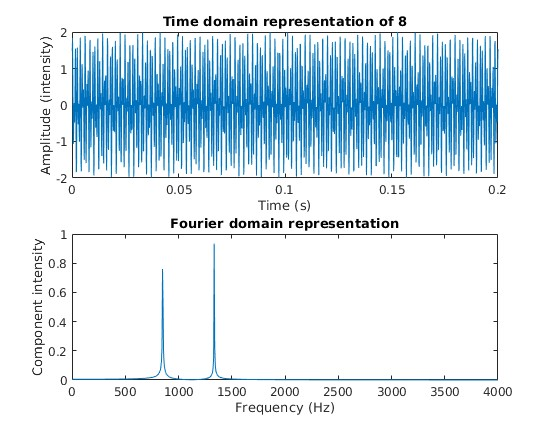
\includegraphics[width =\textwidth]{encode.jpg}
	\label{encode}
	\caption{DTMFencode Time and Fourier Domain}
\end{figure}


\section{Part II}
Since we are making the assumption that only one digit is pressed per recording, we can also assume that it will have the most salient amplitude in the frequency domain.
We could relax this requirement a little bit since we know that the keytone will take one of exactly 12 combinations, and thus focus our attention fully on small intervals around those frequencies.
This should be seriously be taken in consideration for environments that have high frequencies in domains relatively far from DTMF (for example, environments near roads or manufacturing equipment, which can have dominating low noise, or electrical equipment, which can contribute to the high frequency parts of the spectrum).
Here however, we consider a scenario like the 'cocktail party' problem, where the most dominant noise present is in the same part of the spectra as the desired signal.
In this case, we definitely need to make the assumption that the noise is less prevalent than the signal.
This means we can divide the frequency spectrum into two partitions: the $<1000$Hz partition which will be occupied by the 'row' frequencies of DTMF, and the $>1000$Hz part where the 'column' frequencies will live.
Within each of these two regions, we can set a "threshold" at 90\% of the global maximum of the parition, and store the positions of all amplitudes which exceed this threshold.
At this point, the maximum frequencies may not exactly match to the DTMF ones, for a variety of reasons: instead of 1209, they may be 1159, 1212, etc. Instead of finding an exact match, we return the digit which most closely matches (measured as minimum of absolute value 'distance') from the found frequencies.
We also found that it helped to square all datapoints in the frequency domain: this narrows the spikes as shown in figure \ref{normalvssquared}.

We see that doing so significantly reduces the saliency of frequencies that appear to be noise, leaving only the two main spikes with significant amplitudes. While computing even higher orders 

\section{Part III}
We first note that Part III is identical to Part II, with the exception that potentially multiple frequencies may be present in the recording. We of course can't apply part II's algorithm directly, at it will only select one (the most salient) frequency.
With this in mind and the time-domain samples in sight, it is clear that the challenge has boiled down to chopping down the sample into parts, and apply the same algorithm than DTMFencode.
We cant exactly 'find the zeros' since the signal is constantly oscillating between positive and negative. However, we can make an 'envelope" of this signal \ref{envelopedemonstration} and find the zeros (or values close to zero) of \emph{that} function. Because we can safely assume that no digits overlap at the same time, we can cut the signal at these zeros and then pass them pass them individually.
\begin{figure}[h]
	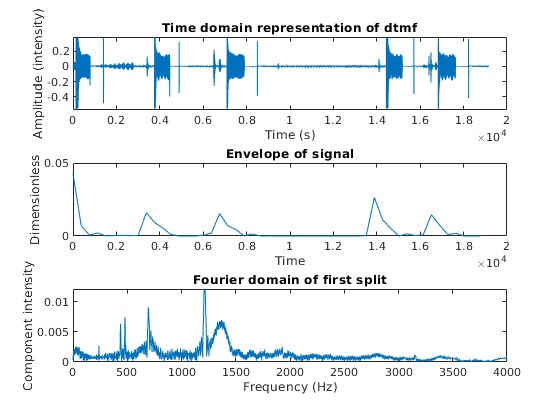
\includegraphics[width =\textwidth]{sequence.jpg}
	\label{envelopedemonstration}
	\caption{Example sequence, envelope, and fourier domain}
\end{figure}

We define this envelope function as $E[x]=\frac{\sum_{k=x-d}^{x+d}f[k]}{2d}$, where d is a parameter to be varied to satisfaction.
Of course, a small value of d will mean that the envelope function is able to discriminate very short spans between the pressing of two numbers, but also means that it might accidentally cut a single frame in two parts if its frequency is low enough.
By squaring the signal to consider only amplitude, we found that d=1 seems to work well for the phone recording. This may seem low at first sight, but considering that the period of a sinusoidal between 900 and 1200Hz is about 9 times higher than default sampling frequency  8000Hz (and nearly double even at 3000Hz, which is our ' worst-case scenario' in this project), it makes sense that the chance of finding 3 consecutive near-0 samples in a nonzero portion of a signal, is very small. Of course this will not be the case for frequencies must lower than this (simply consider points near the y-axis intersection)

\section{Part IV}
Following suggestions from the instructions, we implement a 3-level for loop sequence. The inner loop iterates through all 50 generated audio files with varying duration, weights, and frequency.
We observed a steady, but non-dramatic decrease in accuracy as the noise factor was raised from 0 to 3 in increments of 0.1. The algoritm did start to seriously break down at noise amplitude/original signal amplitude ratio greater than 3.
The cause of deterioration was not so much the Fourier analysis, but finding the "zeros" of the envelope, as shown in figure \ref{noisy}
\begin{figure}[h]
	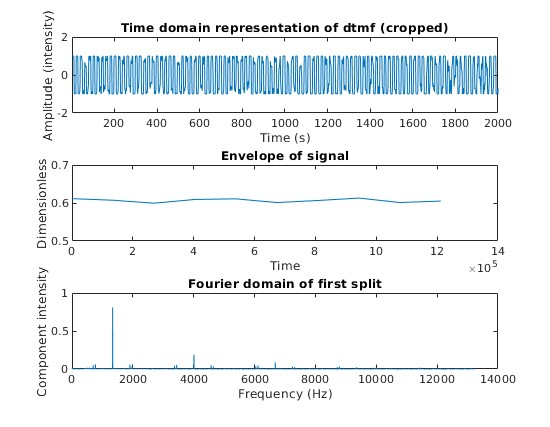
\includegraphics[width =\textwidth]{noisy.jpg}
	\label{noisy}
	\caption{Example sequence "254*603422" with noise factor 3. The envelope hardly differentiates different digits at all: Pay special attention to the y-scale of envelope compared to figure \ref{envelopedemonstration}}
\end{figure}

\begin{figure}[h]
	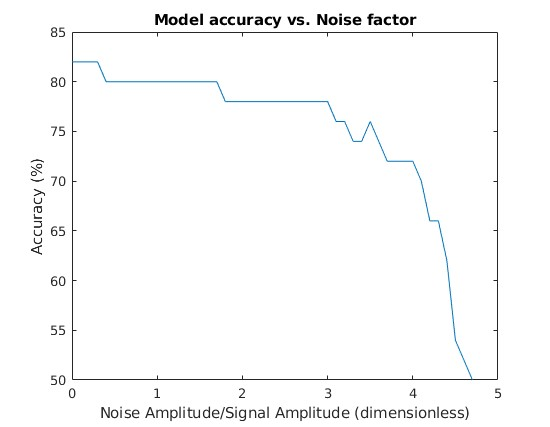
\includegraphics[width =\textwidth]{accuracy.jpg}
	\label{accuracy}
	\caption{Accuracy vs noise}
\end{figure}

\section{Part V}
So far in this investigation, we have assumed that the relative weighting of low and high frequencies are constant thoughout a single sample. In particular, since every tone is composed of exactly one high and one low tone, we expect the amplitude of the signal to be constant across key presses (additive noise nonwithstanding). As is shown clearly in figure \ref{part4enveloper}, this same assumption cannot be made with reverb signals. Figure \ref{reverbacc} shows the accuracy using a naïve implementation, that is, one unmodified from parts I-IV.

There are two primary ways for which the current model is unfit for reverb noise: first, it does not take advantage of the fact that the zeros of the envelope will be very well defined, even at high levels of reverb: this is due to the convolution-based origin of the noise, where 0 convoluted with anything remains 0.
Second, and related to the first, is the fact that we squared the signal in the time domain to get better a sharper understanding of where the digits occurred. Not only is this not necessary, but it is actually counterproductive here, because the amplitude changes across the signal.\\

We should not expect the Fourier Transform of the algorithm to change; multiplication in the time domain is a convolution in the frequency domain, and assuming that the fourier domain is composed of a sum of deltas, they should (at most) be scaled by some factor. This is a transformation to which our algorithm as described in part II stays robust.
\begin{figure}[h]
	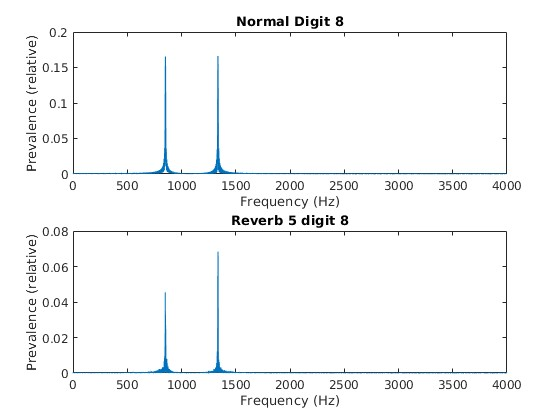
\includegraphics[width =\textwidth]{normalvsreverb.jpg}
	\label{normalvsreverb}
	\caption{As discussed, reverb noise only affects the fourier domain through rescaling of delta spikes}
\end{figure}

\begin{figure}[h]
	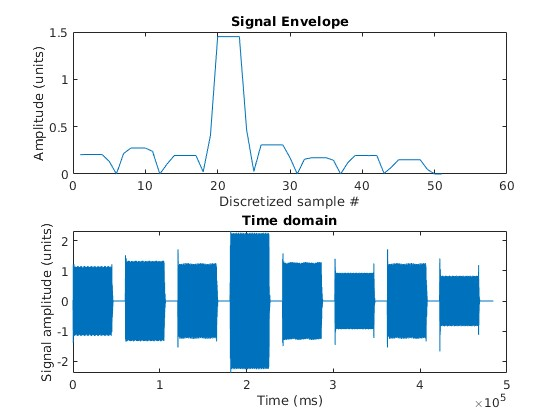
\includegraphics[width =\textwidth]{part4envelope.jpg}
	\label{part4envelope}
	\caption{Computed Envelope and original signal for reverbed signal with duration 1. The squaring of the amplitude (originally meant to reduce additive noise) exacerbates differences in amplitudes in the signal}
\end{figure}
\begin{figure}[h]
	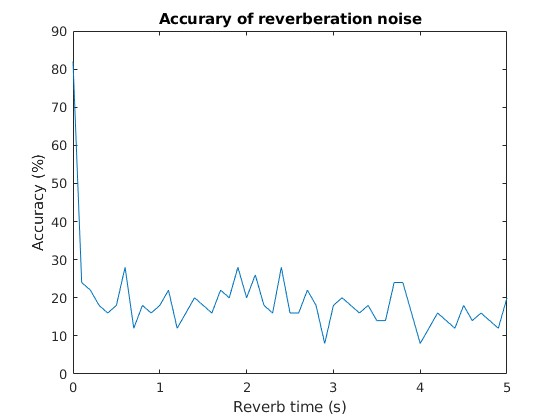
\includegraphics[width =\textwidth]{reverbacc.jpg}
	\label{reverbacc}
	\caption{Naïve model accuracy on the reverbarated dataset.}
\end{figure}


\end{document}
